\documentclass{article}

\usepackage{xcolor}
\usepackage{tikz}
\usepackage{amsthm}
\usepackage{amsmath}
\usepackage{amsfonts}
\usepackage{MnSymbol}
\usetikzlibrary{decorations.pathreplacing}
\usetikzlibrary{calc}
\usetikzlibrary{fit,positioning,hobby}
\usetikzlibrary{decorations.text}


\newtheorem{definition}{Definition}
\newtheorem{example}{Example}

\title{\textbf{CS 355 Topics in Cryptography} \\ Lecture 1}
\author{Edited by ZHENG Tianyu}
\date{23 September 2022}

\begin{document}

\maketitle

\section*{Outline}
\begin{itemize}
    \item What this course is about?
    \item Logistics, administrivia.
    \item Foundations of modern cryptography.
\end{itemize}

\section{What this course is about?}
% TIMELINE - simple test
\vspace{1em}
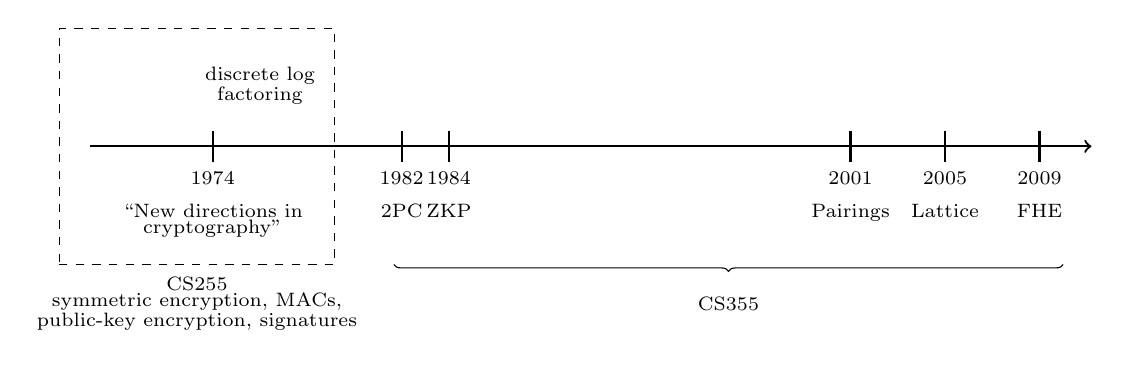
\begin{tikzpicture}[]

\tikzset{
  font={\fontsize{7pt}{6}\selectfont}}
  
  % limits
  \newcount\yearOne; \yearOne=1960
  \def\w{12}    % width of axes
  \def\n{4}     % number of decades
  \def\lt{0.2} %  ten tick length
  \def\lf{0} % five tick length
  \def\lo{0} %  one tick length
 
  % help functions: Label with no year  
  \def\commentLabel(#1,#2){
  \def\x{{(#1-1970)*\w/(\n*10)}}
  \draw[thick] (\x,0) -- (\x,-0) % ten tick
  +(0,\lt*2)node[above,black,align=center] {#2};
  %+(0,\lt*2)node[above] {#1} 
  }
  
  % help functions: Label with year   
  \def\yearLabel(#1,#2){
  \def\x{{(#1-1970)*\w/(\n*10)}}
  \draw[thick] (\x,\lt) -- (\x,-\lt) % ten tick
  node[below] {#1} 
  +(0,-\lt*2)node[below,black,align=center] {#2};
  }
  
  % draw the time axis
  \draw[->,thick] (-\w*0.03,0) -- (\w*1.03,0);

  % label
    \commentLabel(1976, discrete log \\ factoring)
    \yearLabel(1974, ``New directions in \\ cryptography'')
    \yearLabel(1982, 2PC)
    \yearLabel(1984, ZKP)
    \yearLabel(2001, Pairings)    
    \yearLabel(2005, Lattice)        
    \yearLabel(2009, FHE)       
    \node (rect) at (1,0) [draw,dashed,minimum width=3.5cm,minimum height=3cm] {};
    \node at (1,-2) [align=center] {CS255 \\ symmetric encryption, MACs, \\ public-key encryption, signatures};
    \draw[decorate,decoration={brace,mirror}] (3.5, -1.5) -- (12, -1.5);
    \node at (7.75,-2) [align=center] {CS355};
\end{tikzpicture}
\vspace{1em}

We are at an ``inflection'' point in the development of cryptography:
\begin{enumerate}
    \item \underline{Real}, large-scale deployment of ``fancy'' cryptography (i.e beyond public-key cryptography)
    \begin{itemize}
        \item[-] Systems like Zcash (relies on pairing-based cryptography and zero-knowledge proof systems)
    \end{itemize}
    
    \item Potential threat of quantum computers requires re-thinking much of the existing public-key cryptography
    \begin{itemize}
        \item[-] Google recently ran pilot project implementing ring-LWE based key-exchange into Chrome (alongside traditional Diffie-Hellman)
        \item[-] Ongoing NIST competition to standardize new post-quantum cryptography (expect 5-7 years to converge on new standards)
    \end{itemize}
\end{enumerate}

\subsection{Course organization reflects these new developments:}
\begin{enumerate}
    \item Foundations of modern cryptography
    \item Zero-knowledge and protocols
    \item Post-quantum cryptography
    \item Applications of cryptography
\end{enumerate}

\subsection{Our goals in this course:}
\begin{enumerate}
    \item Be your \underline{first} course in advanced cryptography: teach you the foundations of modern cryptography and prepare you to get started with research in cryptography
    \item Be your \underline{last} course in advanced cryptography: give you a taste of the newest development in cryptography and enable you to build the next generation of systems using \underline{cutting-edge} cryptography!
\end{enumerate}

\subsection{Logistics and Administrivia:}
Skip.

\subsection{Foundations of Modern Cryptography:}

Modern cryptography is the study of \underline{hardness}: 

There is some task that should be ``easy'' for an honest party, but ``difficult'' for an adversary,

\begin{example} 
Encryption scheme: given knowledge of the key, it is easy to decrypt, but without the secret key, is is difficult to decrypt.
\end{example} 

\noindent {\color{purple} {Question:How do we model this \underline{mathematically}?}}

This will be very important to develop and understand more advanced concepts. 
In this lecture, we will focus on symmetric primitives.

For our first example, consider a pseudorandom generator (PRG).

\underline{Recall:} A PRG takes a short seed $s$ and expands it into a long ``random-looking'' string:

% TIMELINE - simple test
\vspace{1em}
\begin{tikzpicture}[]
    \node (Sbox) at (0,0) [draw,minimum width=3cm,minimum height=0.6cm] {$s$};
    \node (Gbox) at (0,-1.5) [draw,minimum width=5.5cm,minimum height=0.6cm] {$G(s)$};
    \draw[dashed] (Sbox.south west) -- (Gbox.north west);
    \draw[dashed] (Sbox.south east) -- (Gbox.north east);
    \node at (6,0) [align=center,font=\footnotesize] {$s \in \{0,1\}^{\lambda}$, $\lambda$ is the length of the seed \\ (i.e., security parameter)};
    \node at (6,-1.5) [align=center,font=\footnotesize] {$G(s) \in \{0,1\}^{\ell(\lambda)}$, \\ often called the "stretch" of the PRG \\ {\color{purple} {Question: Why should $\ell(\lambda) > \lambda$}}}
\end{tikzpicture}
\vspace{1em}

\noindent {\color{purple} {Question: What does it mean to be ``random-looking''?}}

\underline{Intuitively:} No efficient algorithm should be able to distinguish it from a truly-random string.

\underline{Formally:} ``efficient'' (for a PRG, seed length = security parameter) will mean \underline{polynomial time} (in the security parameter).

Define distinguishing algorithm as one that takes a string (either output of PRG or truly random string) and guesses whether the string is output of PRG or actual random string.

\begin{definition}
A PRG $G:\{0,1\}^{\lambda} \rightarrow \{0,1\}^{\ell(\lambda)}$ is secure if for all (possibly randomized) algorithms $\mathcal{A}$ running in time $\mathrm{poly}(\lambda)$: 
\end{definition}
                                          
\begin{eqnarray*}
    \left | {\color{red} \mathrm{Pr}[s \overset{\rm R}{\leftarrow} \{0,1\}^{\lambda} : \mathcal{A}(G(s))=1]} - {\color{blue} \mathrm{Pr}[t \overset{\mathrm{R}}{\leftarrow} \{0,1\}^{\ell(\lambda)} : \mathcal{A}(t)=1]} \right |< {\color{purple} \mathrm{negl}(\lambda)},
\end{eqnarray*}

where $s$ is sampled uniformly from $\{0,1\}^{\lambda}$, and
\begin{enumerate}
\item ${\color{red} \mathrm{Pr}[s \overset{\rm R}{\leftarrow} \{0,1\}^{\lambda} : \mathcal{A}(G(s))=1]}$: adversary sees output of PRG on random seed. 

\item ${\color{blue} \mathrm{Pr}[t \overset{\rm R}{\leftarrow} \{0,1\}^{\ell(\lambda)} : \mathcal{A}(t)=1]}$: adversary sees totally random string.

\item ${\color{purple} \mathrm{negl}(\lambda)}$: a function $f(\lambda)$ is negligible in $\lambda$ if $f(\lambda) = \mathcal{O}(\frac{1}{\lambda^c})$ for all constants $c \in N$.
\end{enumerate}

Intuitively: behavior of algorithm $\mathcal{A}$ does not vary much on PRG outputs and truly random outputs.

Oftentimes, we define following variables:
\begin{eqnarray}
    & W_0 = {\color{red}\mathrm{Pr}[s \overset{\mathrm{R}}{\leftarrow} \{ 0,1 \}^{\lambda}: \mathcal{A}(G(s))=1]}, & \text{``pseudorandom''} \nonumber\\
    & W_1 = {\color{blue}\mathrm{Pr}[t \overset{\mathrm{R}}{\leftarrow} \{ 0,1 \}^{\ell(\lambda)}: \mathcal{A}(t)=1]}. & \text{``random''} \nonumber
\end{eqnarray}

The PRG distinguishing advantage is then $\mathrm{PRGAdv}[\mathcal{A},G] = |W_0-W_1|$.

We can also view this definition through the lens of computational indistinguishability.
\begin{definition}
Let $\lambda \in \mathbb{N}$ be a security parameter. Let $D_1 = \{ D_{1,\lambda} \}_{\lambda \in \mathbb{N}}$ and $D_2 = \{ D_{2,\lambda} \}_{\lambda \in \mathbb{N}}$ be collections (ensembles) of distributions indexed by $\lambda$. Then, $D_1$ and $D_2$ are computationally indistinguishable (denoted $D_1 {\approx}^{c} D_2$) if for all efficient adversaries $\mathcal{A}$,
\begin{eqnarray*}
    |\mathrm{Pr}[x_1 \leftarrow D_{1,\lambda}:\mathcal{A}(1^{\lambda},x_1)=1] - \mathrm{Pr}[x_2 \leftarrow D_{2,\lambda}:\mathcal{A}(1^{\lambda},x_2)=1]| = \mathrm{negl}(\lambda).
\end{eqnarray*}
\end{definition}

\begin{definition}
(PRG security definition) $G: \{ 0,1 \}^{\lambda} \rightarrow \{ 0,1 \}^{\ell(\lambda)}$ is a secure PRG if $D_1 {\approx}^{c} D_2$ where 
\begin{eqnarray*}
     D_1 &=& \{ s \overset{\mathrm{R}}{\leftarrow} \{ 0,1 \}^{\lambda}: G(s) \}, \nonumber \\
     D_2 &=& \{ t \overset{\mathrm{R}}{\leftarrow} \{ 0,1 \}^{\ell(\lambda)}: t \}. \nonumber 
\end{eqnarray*}
\end{definition}

\noindent {\color{purple} {Question: Do PRGs exist?}} 

Unknown! Requires (minimally) resolving $\mathcal{P} \text{ vs. } \mathcal{NP}$.
But if one-way functions (OWFs) exist, then we can build PRG that expand by a single bit: $\ell(\lambda) = \lambda+1$ (Will explore this on HW1, Problem 2)
\\

\noindent {\color{purple} {Question: How to go from one-bit PRG to multi-bit PRG?}} 

\underline{Blum-Micali PRG:} Suppose we have PRG $\mathcal{G}$ that expands by 1-bit:

\input{Lec1-3.tex}

We can iterate $m$ times to obtain $m$ output bits.
\\

\noindent {\color{purple} {Question: Is this construction secure?}} 

To prove security, we will use a \underline{``hybrid'' argument}.

Suppose we iterate Blum-Micali $m$ times. We need to show that the following distributions are computationally indistinguishable:
\begin{eqnarray*}
    D_1 &=& \{ s_0 \overset{\mathrm{R}}{\leftarrow} \{ 0,1 \}^{\lambda}: H(s_0) \}, \nonumber \\
    D_2 &=& \{ t \overset{\mathrm{R}}{\leftarrow} \{ 0,1 \}^{m}: t \}, \nonumber 
\end{eqnarray*}
where $H(s_0)$ is $m$ iterations of Blum-Micali.

Define intermediate distributions $D_{1,i}$ for $i=0,...,m$ as following figure.

Let $p_{1,0} = \mathrm{Pr}[x\leftarrow D_{1,0}:\mathcal{A}(x)=1]$ ... $p_{1,m} = \mathrm{Pr}[x\leftarrow D_{1,m}:\mathcal{A}(x)=1]$ then,
\begin{align*} 
    \mathrm{PRGAdv}[\mathcal{A},H] =& \left| p_{1,0}-p_{1,m} \right| 
    \\
    =& \left| p_{1,0}-p_{1,1} + p_{1,1}-p_{1,2} + \cdots + p_{1,m}-p_{1,m} \right|
    \\
    \leq& \left| p_{1,0}-p_{1,1} \right| + \left| p_{1,1}-p_{1,2} \right| + \cdots + \left| p_{1,m}-p_{1,m} \right| \text{  by triangle inequality}
\end{align*}

\underline{Observe:} Quantity $\left| p_{1,0}-p_{1,1} \right|$ is essentially distinguishing advantage of some algorithm for $\mathcal{G}$.

\vspace{1em}
\begin{center}
\begin{tikzpicture}[trafo/.style={midway,font=\tiny}]

  \def\hd{1}\def\vd{1}

  \def\arrowdraw(#1,#2){
  \draw[->] ($ (#1) + (\hd/3,0) $) -- ($ (#2) + (-\hd/3,0) $);
  }
  
\def\darrowdraw(#1,#2){
  \draw[->] ($ (#1) + (0,-\hd/3) $) -- ($ (#2) + (0,\hd/3) $);
  }
  
  % Row 1
  \node (case1) at (-2,0) {$D_1 = D_{1,0}$};
  \node (S0) at (0,0) {$S_0$};
  \node[right=\hd of S0, draw] (G1) {$\mathcal{G}$};
  \node[right=\hd of G1] (S1) {$S_1$};
  \node[right=\hd of S1, draw] (G2) {$\mathcal{G}$};
  \node[right=\hd of G2] (S2) {$S_2$};
  \node[right=\hd of S2, draw] (G3) {$\mathcal{G}$};
  \node[right=\hd of G3] (more) {$\cdots$};

  
  \node[below=\vd of G1] (b1) {$b_1$};
  \node[below=\vd of G2] (b2) {$b_2$};
  \node[below=\vd of G3] (b3) {$b_3$};
  
  \arrowdraw(S0,G1);
  \arrowdraw(G1,S1);
  \arrowdraw(S1,G2);
  \arrowdraw(G2,S2);
  \arrowdraw(S2,G3);
  \arrowdraw(G3,more);
  
  \darrowdraw(G1,b1);
  \darrowdraw(G2,b2);
  \darrowdraw(G3,b3);
  
  % Row 2
  \node[below=\vd*2 of case1] (case2) {$D_{1,1}$};
  \node[below=\vd of S0] (S0-2) {\color{red}\footnotesize $S_0 \overset{\mathrm{R}}{\leftarrow} \{0,1\}^{\lambda}$};
  
  \node[below=\vd*2 of S1] (S1-2) {\color{green} $S_1$};
  \node[right=\hd of S1-2, draw] (G2-2) {$\mathcal{G}$};
  \node[right=\hd of G2-2] (S2-2) {$S_2$};
  \node[right=\hd of S2-2, draw] (G3-2) {$\mathcal{G}$};
  \node[right=\hd of G3-2] (more-2) {$\cdots$};
  
  \node[below=\vd of G2-2] (b2-2) {$b_2$};
  \node[below=\vd of G3-2] (b3-2) {$b_3$};

  \arrowdraw(S1-2,G2-2);
  \arrowdraw(G2-2,S2-2);
  \arrowdraw(S2-2,G3-2);
  \arrowdraw(G3-2,more-2);
  
  \darrowdraw(G2-2,b2-2);
  \darrowdraw(G3-2,b3-2);
  
  % Row 3
  \node[below=\vd*2 of case2] (case3) {$D_{1,2}$};
  \node[below=\vd*3 of G1, align=center] (S1-3) {\color{red}\footnotesize $b_1 \overset{\mathrm{R}}{\leftarrow} \{0,1\}$ \\\color{red}\footnotesize $S_1 \overset{\mathrm{R}}{\leftarrow} \{0,1\}^{\lambda}$};
  
  \node[below=\vd*2 of S2-2] (S2-3) {\color{green} $S_2$};
  \node[right=\hd of S2-3, draw] (G3-3) {$\mathcal{G}$};
  \node[right=\hd of G3-3] (more-3) {$\cdots$};
  
  \node[below=\vd of G3-3] (b3-3) {$b_3$};

  \arrowdraw(S2-3,G3-3);
  \arrowdraw(G3-3,more-3);
  
  \darrowdraw(G3-3,b3-3);
  
  % Row 4
  \node[below=\vd*0.55 of case3] (case4) {$\vdots$};
  \node[below=\vd*5 of G1, align=center] (S1-4)
  {\color{red}\footnotesize $b_1 \overset{\mathrm{R}}{\leftarrow} \{0,1\}$};
  \node[below=\vd*5 of G2, align=center] (S2-4)
  {\color{red}\footnotesize $b_2 \overset{\mathrm{R}}{\leftarrow} \{0,1\}$
  \\\color{red}\footnotesize $S_2 \overset{\mathrm{R}}{\leftarrow} \{0,1\}^{\lambda}$};
  
  % Row 5
  \node[below=\vd*0.55 of case4] (case5) {$D_2 = D_{1,m}$};
  \node[below=\vd*7 of G1, align=center] (S1-5)
  {\color{red}\footnotesize $b_1 \overset{\mathrm{R}}{\leftarrow} \{0,1\}$};
  \node[below=\vd*7 of G2, align=center] (S2-5)
  {\color{red}\footnotesize $b_2 \overset{\mathrm{R}}{\leftarrow} \{0,1\}$};
  \node[below=\vd*7 of more, align=center] (S3-5)
  {\\ \color{red}\footnotesize $\cdots$};
  \node[right=\hd of S3-5, align=center] (S3-5)
  {\\ \color{red}\footnotesize $b_m \overset{\mathrm{R}}{\leftarrow} \{0,1\}$};
  
\end{tikzpicture}
\end{center}

More precisely, suppose $\left| p_{1,0} - p_{1,1} \right| = \epsilon$. We use $\mathcal{A}$ to build distinguisher $\mathcal{B}$ for $\mathcal{G}$ such that distinguisher $\mathcal{B}$ works as follows: 
\begin{enumerate}
    \item On input a string $z \in \{ 0,1 \}^{\lambda+1}$, $\mathcal{B}$ parses $z = (b_1, s_1)$
    \item Algorithm $\mathcal{B}$ computes
    \vspace{1em}
\begin{center}
\begin{tikzpicture}[trafo/.style={midway,font=\tiny}]

  \def\hd{1}\def\vd{1}

  \def\arrowdraw(#1,#2){
  \draw[->] ($ (#1) + (\hd/3,0) $) -- ($ (#2) + (-\hd/2.5,0) $);
  }
  
\def\darrowdraw(#1,#2){
  \draw[->] ($ (#1) + (0,-\vd/3) $) -- ($ (#2) + (0,\vd/3) $);
  }
  
  \node (S0) at (0,0) {$S_1$};
  \node[right=\hd of S0, draw] (G1) {$\mathcal{G}$};
  \node[right=\hd of G1] (S1) {$S_2$};
  \node[right=\hd of S1, draw] (G2) {$\mathcal{G}$};
  \node[right=\hd of G2] (more) {$\cdots$};
  \node[right=\hd of more, draw] (G3) {$\mathcal{G}$};
  \node[right=\hd of G3] (S2) {$S_{n+1}$};
  
  \node[below=\vd of G1] (b1) {$b_2$};
  \node[below=\vd of G2] (b2) {$b_3$};
  \node[below=\vd of G3] (b3) {$b_n$};

  \arrowdraw(S0,G1);
  \arrowdraw(G1,S1);
  \arrowdraw(S1,G2);
  \arrowdraw(G2,more);
  \arrowdraw(more,G3);
  \arrowdraw(G3,S2);
  
  \darrowdraw(G1,b1);
  \darrowdraw(G2,b2);
  \darrowdraw(G3,b3);
\end{tikzpicture}
\end{center}
    and invokes $\mathcal{A}$ on inputs $b_1,...,b_n$
    \item Algorithm $\mathcal{B}$ outputs whatever $\mathcal{A}$ outputs
\end{enumerate}

Tow case to consider:
\begin{enumerate}
    \item[-] if $(b_1,s_1) \leftarrow G(s)$ where $s \leftarrow \{ 0,1 \}^{\lambda}$, then $\mathcal{A}$ outputs 1 with probability $p_{1,0}$ (by definition of $D_{1,0}$)
    \item[-] if $(b_1,s_1) \overset{\mathrm{R}}{\leftarrow} \{ 0,1 \}^{\lambda+1}$, $\mathcal{A}$ outputs 1 with probability $p_{1,1}$ (by definition of $D_{1,1}$)
\end{enumerate}
Thus, $\mathrm{PRGAdv}[\mathcal{B},\mathcal{G}] = \left| p_{1,0} - p_{1,1} \right| = \epsilon$. \qquad $ \blacksquare$ 
\\

\noindent \underline{Conclusion:} We can bound each $\left| p_{1,i} - p_{1,i+1} \right|$ by $\mathrm{PRGAdv}[\mathcal{B},\mathcal{G}]$ for some efficient distinguisher $\mathcal{B}$. Thus, 
\begin{equation*}
    \mathrm{PRGAdv}[\mathcal{A},\mathcal{H}] \leq m \cdot \mathrm{PRGAdv}[\mathcal{B},\mathcal{G}],
\end{equation*}
since $\mathcal{G}$ is a secure PRG and $\mathcal{B}$ is efficient, 
\begin{equation*}
\mathrm{PRGAdv}[\mathcal{B},\mathcal{G}] = \mathrm{negl}(\lambda),
\end{equation*}
so as long as $m = \mathrm{poly}(\lambda)$, 
\begin{equation*}
\mathrm{PRGAdv}[\mathcal{A},\mathcal{H}] \leq m \cdot \mathrm{PRGAdv}[\mathcal{B},\mathcal{G}] = m \cdot \mathrm{negl}(\lambda) = \mathrm{negl}(\lambda). \qquad \blacksquare
\end{equation*}

\noindent \underline{General hybrid argument approach:} to argue indistinguishability of two distributions: 
\begin{enumerate}
    \item Identify sequence of intermediate distributions between the target distributions
    \item Argue that each consecutive pair of hybrid distributions are computationally indistinguishable
\end{enumerate}

More abstractly: 
if $D_1 {\approx}^{c} D_2 {\approx}^{c} \cdots {\approx}^{c} D_m$ and $m = \mathrm{poly}(\lambda)$, then $D_1 {\approx}^{c} D_m$ (computational indistinguishability is essentially transitive).
\\

\noindent \underline{Other symmetric primitives (review):}

\textbf{Pseudorandom functions (PRFs):} A PRF $\mathrm{F}: \mathcal{K} \times \mathcal{X} \rightarrow \mathcal{Y}$ (strictly speaking, $\mathcal{K},\mathcal{X},\mathcal{Y}$ are all ensembles indexed by $\lambda$) on a key space $\mathcal{K}$, domain $\mathcal{X}$ and range $\mathcal{Y}$ if for all efficient adversaries $\mathcal{A}$, 
\begin{equation*}
    \mathrm{PRGAdv}[\mathcal{A},\mathrm{F}] = \left| \mathrm{Pr}[W_0=1] - \mathrm{Pr}[W_1=1] \right| = \mathrm{negl}(\lambda)
\end{equation*}

where for $b \in \{ 0,1 \}$, we define $W_b$ as output of $\mathcal{A}$ in the following experiment:

\vspace{1em}
\begin{center}
\begin{tikzpicture}[>=latex]
    \node[draw,rectangle,minimum width = 4cm,minimum height = 3cm] (A) at (-3.5,0) {};
    \node[draw,rectangle,minimum width = 4cm,minimum height = 3cm] (C) at (3.5,0) {};
    
    \draw[->] (line1) ($ (A) + (2.7,0.5) $) -- ($ (C) + (-2.7,0.5) $);
    \draw[->] (line2) ($ (C) + (-2.7,-0.5) $) -- ($ (A) + (2.7,-0.5) $);
    
    \node[above=0 of A] (adv) {adversary};
    \node[above=0 of C] (cha) {challenger};
    \node[above=0.5 of line1] (m1) {$x \in \mathcal{X}$};
    \node[above=-0.5 of line2] (m2) {$y$};
    
    \node[above=-1.5 of A] (Astep) {$b' \in \{ 0,1 \}$};
    \node[above=-2.5 of C, align = center] (Cstep) {
    if $b=0: k \leftarrow \mathcal{K}$ \\ 
    if $b=1: f \overset{\mathrm{R}}{\leftarrow} \mathrm{Funs}[\mathcal{X},\mathcal{Y}]$ \\
    if $b=0: y \leftarrow \mathrm{F}(k,x)$ \\
    if $b=1: y \leftarrow \mathrm{f}(x)$
    };
    
\end{tikzpicture}
\end{center}
\vspace{1em}

In particular, $\mathcal{A}$ can not distinguish outputs of PRF from that of a \underline{truly random} function.

\textbf{Pseudorandom permutations (PRPs):} Similar to PRFs except replace function with permutation.

\textbf{One-way functions (OWFs):} A function $f:\mathcal{X}_{\lambda} \leftarrow \mathcal{Y}_{\lambda}$ is one-way if for all efficient adversaries $\mathcal{A}$:
\begin{equation*}
    \mathrm{Pr}[x \leftarrow \mathcal{X}_{\lambda}: f(\mathcal{A}(f(x)))=x] = \mathrm{negl}(\lambda)
\end{equation*}

\underline{Intuitively:} One-way functions are difficult to invert.
\\

Connections between symmetric primitives:

\vspace{1em}
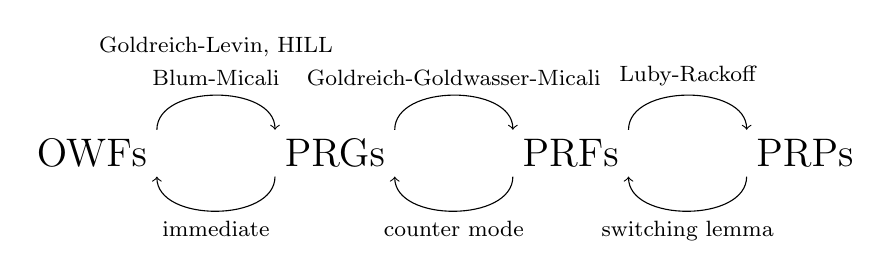
\begin{tikzpicture}
  \node (OWF) at (0,0) {\Large OWFs};
  \node[right = 1.5 of OWF] (PRG) {\Large PRGs};
  \node[right = 1.5 of PRG] (PRF) {\Large PRFs};
  \node[right = 1.5 of PRF] (PRP) {\Large PRPs};
  
  \draw[->] (OWF.north east) to [out=90,in=90, edge node={node [above, align = center] {\footnotesize Goldreich-Levin, HILL \\\footnotesize Blum-Micali}}] (PRG.north west);
  \draw[->] (PRG.north east) to [out=90,in=90, edge node={node [above, align = center] {\footnotesize Goldreich-Goldwasser-Micali}}] (PRF.north west);
  \draw[->] (PRF.north east) to [out=90,in=90, edge node={node [above, align = center] {\footnotesize Luby-Rackoff}}] (PRP.north west);

  \draw[->] (PRP.south west) to [out=270,in=270, edge node={node [below, align = center] {\footnotesize switching lemma}}] (PRF.south east);
  \draw[->] (PRF.south west) to [out=270,in=270, edge node={node [below, align = center] {\footnotesize counter mode}}] (PRG.south east);
  \draw[->] (PRG.south west) to [out=270,in=270, edge node={node [below, align = center] {\footnotesize immediate}}] (OWF.south east);
\end{tikzpicture}
\vspace{1em}

Implication: OWFs is minimal assumption for symmetric cryptography.
\\

{\color{purple} [If there is time: Goldreich-Goldwasser-Micali: PRF from PRG]}

Suppose we have a length doubling PRG $\mathcal{G}:\{ 0,1 \}^{\lambda} \leftarrow \{ 0,1 \}^{2\lambda}$ 
\begin{eqnarray*}
    \text{Construction:} & & \mathcal{K}_{\lambda} = \{ 0,1 \}^{\lambda} \\ 
    & & \mathcal{X}_{\lambda} = \{ 0,1 \}^{n(\lambda)} \\ 
    & & \mathcal{Y}_{\lambda} = \{ 0,1 \}^{\lambda} \\ 
    \text{Write:} & & \mathcal{G}(s) \leftarrow (s_0,s_1) = (\mathcal{G}_0(s),\mathcal{G}_1(s)) \\
    \text{Then,} & & \text{PRF value at } x_1,...,x_n \text{ is } \mathcal{G}_{x_n}(\mathcal{G}_{x_{n-1}}(\cdots \mathcal{G}_{x_1}(s) \cdots)) \\ 
\end{eqnarray*}

Picture (when $n=2$):
% TIMELINE - simple test
\vspace{1em}
\begin{center}
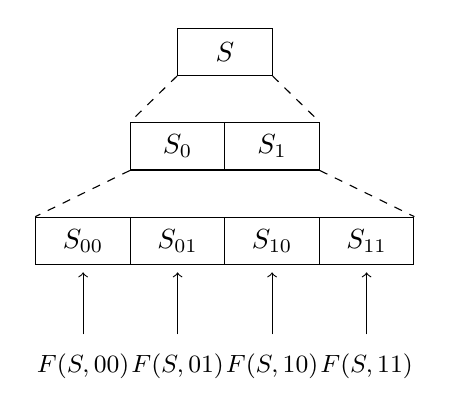
\begin{tikzpicture}
    \def\hd{1.2cm}
    \def\arrowdraw(#1,#2){
    \draw[->] ($ (#1) + (0,\hd/3) $) -- ($ (#2) + (0,-\hd/3) $);
    }
  
    \node (Sbox) at (0,0) [draw,minimum width=\hd,minimum height=0.5*\hd] {$S$};
    
    \node (S0box) at (-0.5*\hd,-\hd) [draw,minimum width=\hd,minimum height=0.5*\hd] {$S_0$};
    \node (S1box) at (0.5*\hd,-\hd) [draw,minimum width=\hd,minimum height=0.5*\hd] {$S_1$};
    
    \node (S00box) at (-1.5*\hd,-2*\hd) [draw,minimum width=\hd,minimum height=0.5*\hd] {$S_{00}$};
    \node (S01box) at (-0.5*\hd,-2*\hd) [draw,minimum width=\hd,minimum height=0.5*\hd] {$S_{01}$}; 
    \node (S10box) at (0.5*\hd,-2*\hd) [draw,minimum width=\hd,minimum height=0.5*\hd] {$S_{10}$};
    \node (S11box) at (1.5*\hd,-2*\hd) [draw,minimum width=\hd,minimum height=0.5*\hd] {$S_{11}$}; 
    
    \node[below=1 of S00box] (F00) {\small $F(S,00)$};
    \node[below=1 of S01box] (F01) {\small $F(S,01)$};
    \node[below=1 of S10box] (F10) {\small $F(S,10)$};
    \node[below=1 of S11box] (F11) {\small $F(S,11)$};
    
    \draw[dashed] (Sbox.south west) -- (S0box.north west);
    \draw[dashed] (Sbox.south east) -- (S1box.north east);
    \draw[dashed] (S0box.south west) -- (S00box.north west);
    \draw[dashed] (S1box.south east) -- (S11box.north east);   
    
    \arrowdraw(F00,S00box)
    \arrowdraw(F01,S01box)
    \arrowdraw(F10,S10box)
    \arrowdraw(F11,S11box)
    
\end{tikzpicture}
\end{center}
\vspace{1em}
Security proof is another hybrid argument (left as exercise)
\end{document}
